\documentclass{article}
\usepackage{graphicx, amsfonts, amssymb, amsmath, amsthm, float, subcaption} % Required for inserting images
\usepackage[english]{babel}
\usepackage[letterpaper,top=2cm,bottom=2cm,left=3cm,right=3cm,marginparwidth=1.75cm]{geometry}

\title{EE132 Lab 3}
\author{Andre Winkel, Russell Yang}
\date{\today}

\begin{document}
\maketitle

\begin{abstract}
    In this lab, we will analyze the stability of different systems. We will observe the open-loop position and speed response in order to determine and reaffirm our definitions for system stability. We will do so by verifying that any bounded input result in a bounded output, which is our definition of [BIBO] stability.
\end{abstract}

\section{System built} 
\begin{figure} [H]
    \centering
    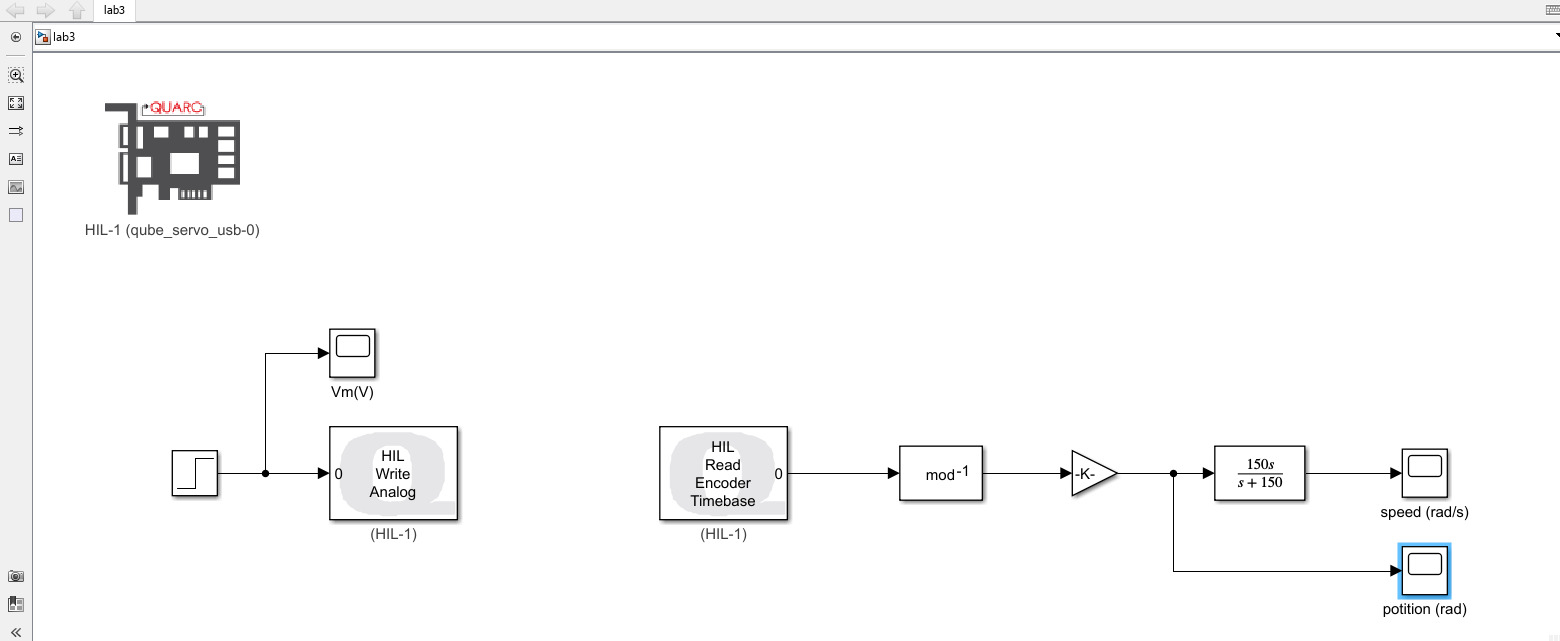
\includegraphics[width=0.75\linewidth]{system.png}
    \caption{Simulink model constructed for this lab}
    \label{fig:1}
\end{figure}
When changing the system's input, we will modify the input connected to \verb|HIL Write Analog| and the voltage scope \verb|Vm(V)|.

\section{In-Lab exercises and Results}
\subsection{Stability of the voltage-to-speed system}
We can determine the stability of the voltage-to-speed system through analyzing the poles of our transfer function,
\begin{equation}
    P_{v-s}(s)=\frac{\Omega_m(s)}{V_m(s)}=\frac{K}{\tau s+1},
\end{equation}
where we have $K=23.0 \frac{\text{rad}}{\text{s}}$ as the steady-state gain, $\tau=0.13\text{s}$ as the time constant, $\Omega_m(s)=\mathcal{L}\{\omega_m(t)\}$ as the motor speed, and $V_m(s)=\mathcal{L}\{v_m(t)\}$ as the applied motor voltage. We can determine the stability of the voltage-to-speed system by analyzing the poles of the transfer function. The poles of this first-order system lie in 
\begin{equation}
    s=-\frac{1}{\tau}, 
\end{equation}
which is in the left half of the complex plane. Considering this, $\tau$ being positive, as well as how it is inherently a causal LTI system, the system is BIBO stable.

\subsection{Stability of the voltage-to-position system}
We can determine the stability of the voltage-to-position system through the poles of our transfer function,
\begin{equation}
    P(s)=P_{v-p}=\frac{\Theta_m(s)}{V_m(s)}=\frac{K}{s(\tau s+1)},
\end{equation}
which is the same as the previous transfer function with an integrator in series, and where $\Theta_m(s)=\mathcal{L}\{\theta_m(t)\}$ is the load gear position. Analyzing the transfer function for stability, we see the poles of this second-order system lie in
\begin{equation}
    s=0,-\frac{1}{\tau}.
\end{equation}
As we have a pole at $s=0$, we can determine that the system will not decay to zero for a bounded input. Therefore, a bounded input can cause a bounded output, meaning this system is not BIBO stable.

\subsection{Applying a unit step voltage}
Here, we apply a unit step voltage to the servo by running our QUARC model.
\begin{figure}[H]
    \centering
    \begin{subfigure}[b]{0.45\linewidth}
        \centering
        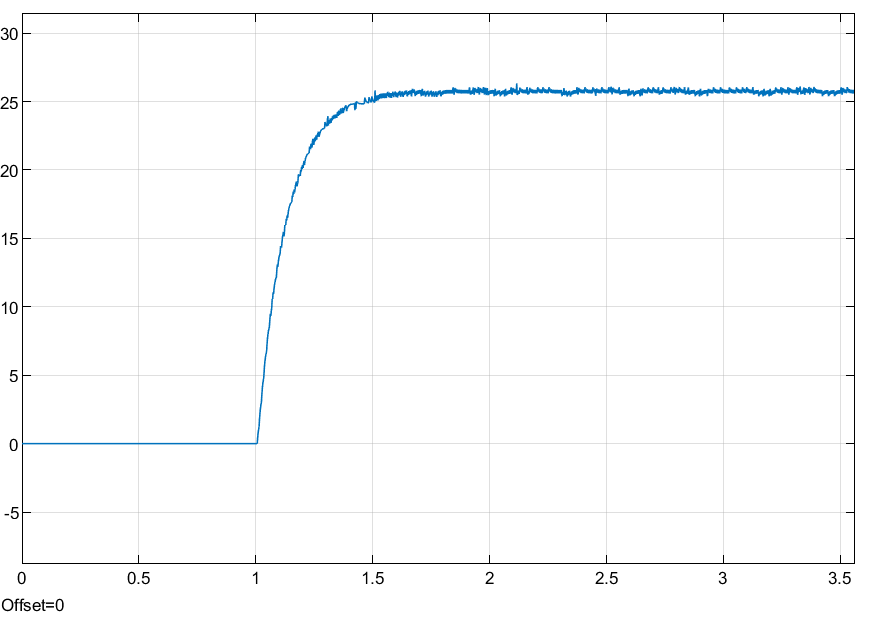
\includegraphics[width=\linewidth]{speed.png}
        \caption{Speed response}
        \label{fig:speed}
    \end{subfigure}
    \hfill
    \begin{subfigure}[b]{0.45\linewidth}
        \centering
        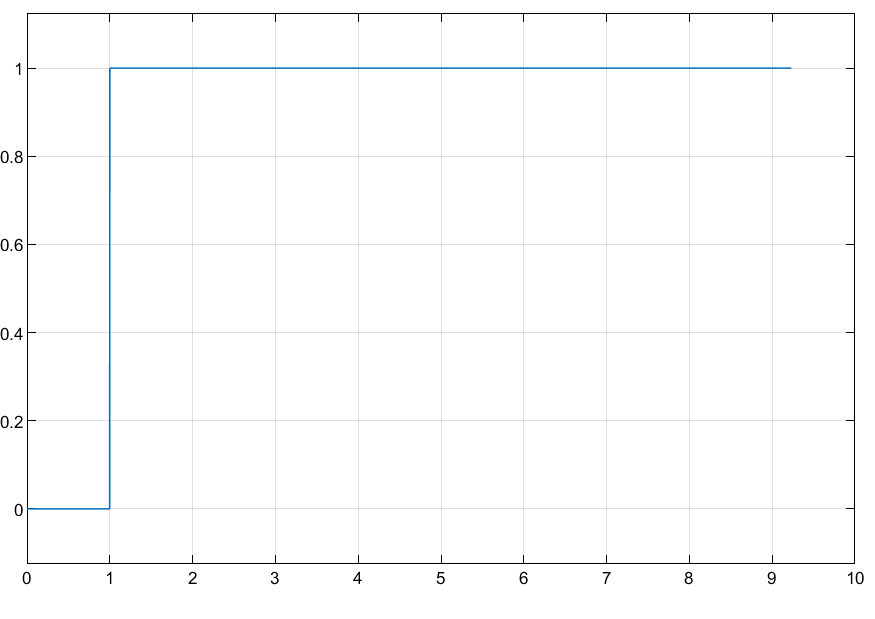
\includegraphics[width=\linewidth]{voltage.png}
        \caption{Voltage input}
        \label{fig:voltage}
    \end{subfigure}
    \\[\baselineskip]
    \begin{subfigure}[b]{0.45\linewidth}
        \centering
        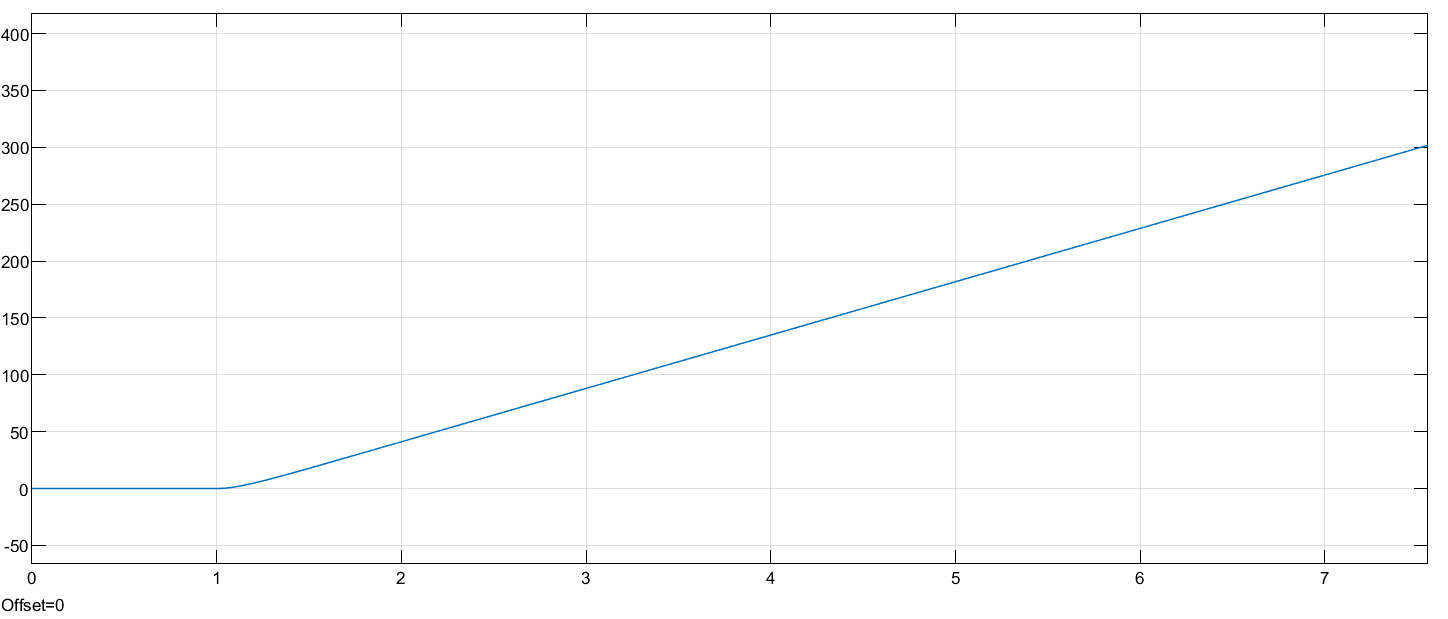
\includegraphics[width=\linewidth]{position.png}
        \caption{Position response}
        \label{fig:position}
    \end{subfigure}
    \caption{System response to unit step input}
    \label{fig:unitstep}
\end{figure}

\subsection{Analysis of speed and position stability}
Based on the plots of the system, we can observe BIBO stability in the speed response with respect to the unit step input. On the other hand, the position response is not stable and appears to approach infinity as $t\to\infty$. Both of these conclusions are in line with our original analysis.

\subsection{BIBO stability based on position response}
We observe from the plots that the position response of the system is unbounded as $t\to\infty$, though our input (unit step) is bounded. This conclusion is, once again, the same as our original analysis.

\subsection{Input for position response stability}
We attempted multiple methods of achieving this. Our initial success was using a sinusoidal function as our voltage input because it directly influences the position output, and we assumed that the periodic nature of a sine wave would prevent unbounded drift. The plots for this input are pictured below:
\begin{figure}[H]
    \centering
    \begin{subfigure}[b]{0.45\linewidth}
        \centering
        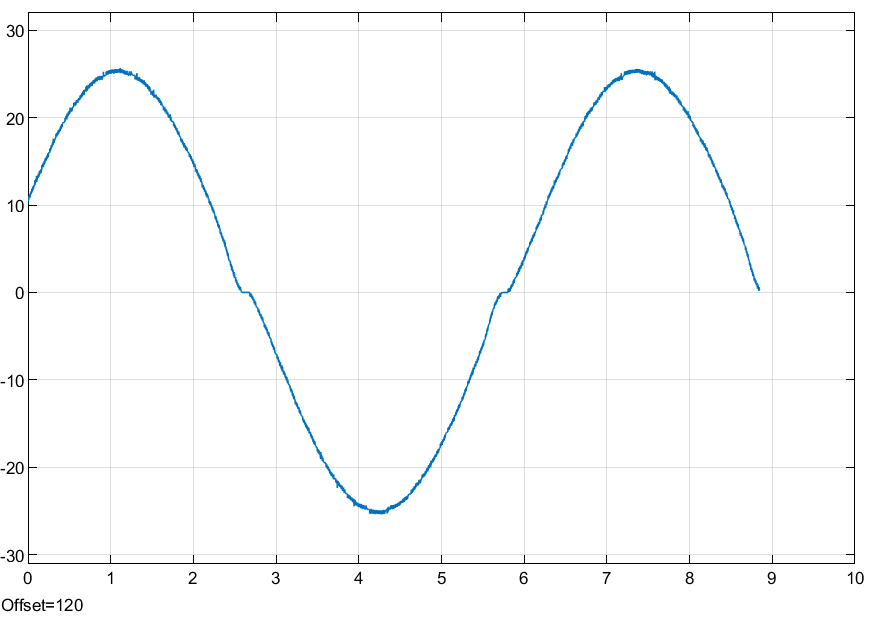
\includegraphics[width=\linewidth]{sinespeed.png}
        \caption{Sinusoidal speed response}
        \label{fig:sinespeed}
    \end{subfigure}
    \hfill
    \begin{subfigure}[b]{0.45\linewidth}
        \centering
        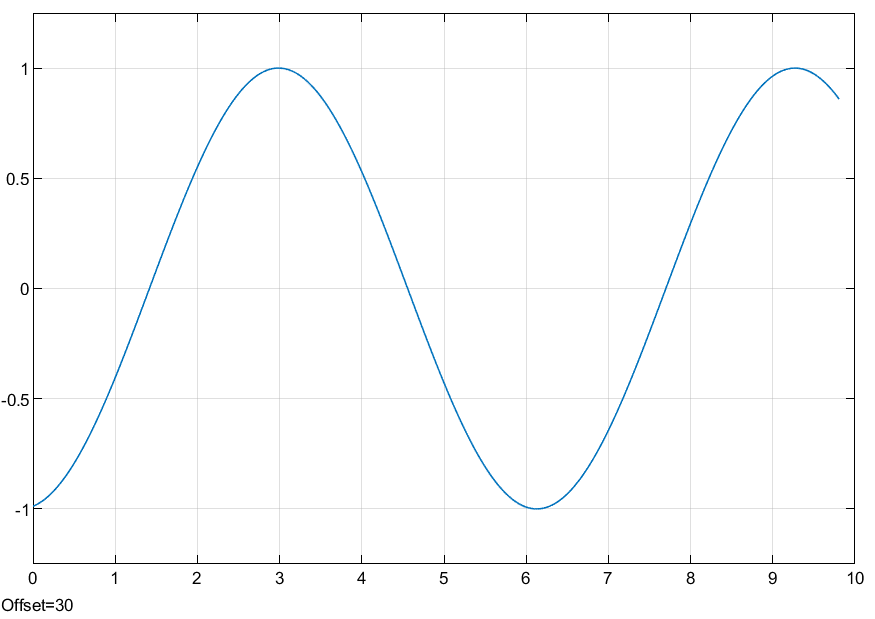
\includegraphics[width=\linewidth]{sinevoltage.png}
        \caption{Sinusoidal voltage input}
        \label{fig:sinevoltage}
    \end{subfigure}
    \\[\baselineskip]
    \begin{subfigure}[b]{0.45\linewidth}
        \centering
        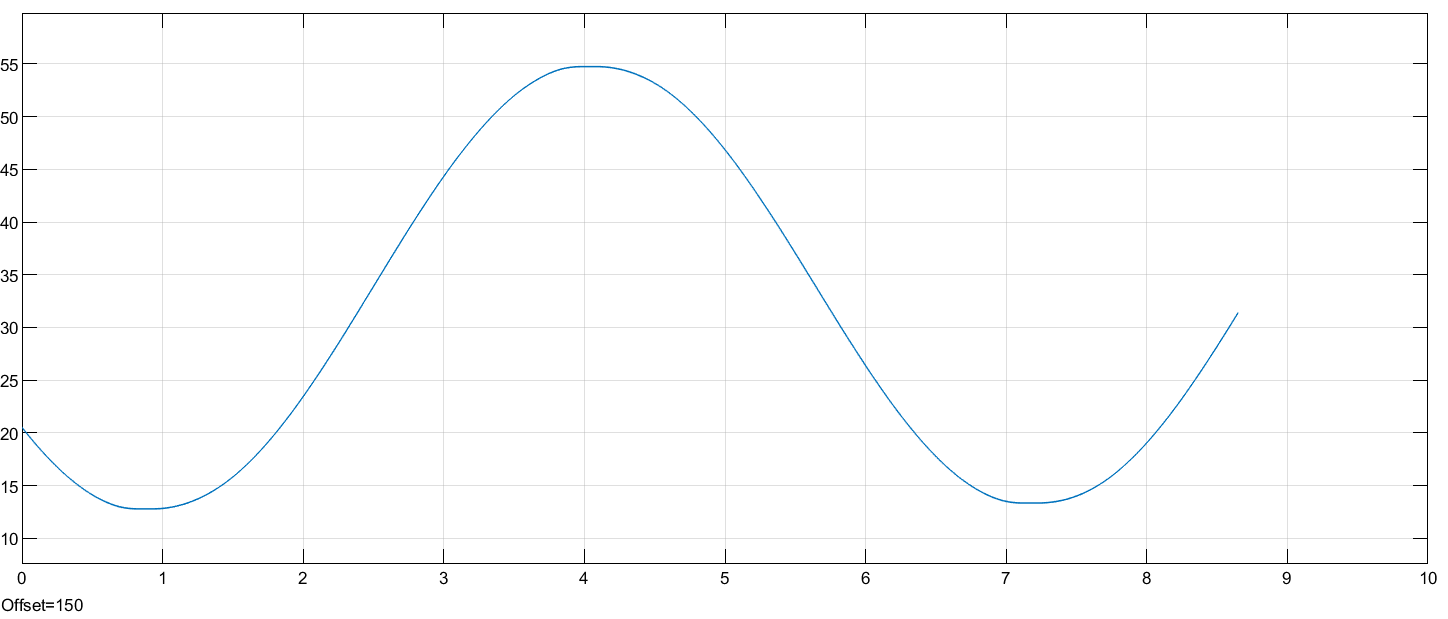
\includegraphics[width=\linewidth]{sinepos.png}
        \caption{Sinusoidal position response}
        \label{fig:sisepos}
    \end{subfigure}
    \caption{System response to sinusoidal input}
    \label{fig:sine}
\end{figure}
\noindent We can directly observe that the position response $p_m(t) \le B$ for some finite $B$ when a pure sinusoidal voltage input is applied. The primary logic behind this is that a pure sinusoid's integral will be 0 across $\mathbb{R}$. This aligns with the fact that an integrator accumulates the area under the input signal. Therefore, any input $v_m(t)$ satisfying
\begin{equation}
    \int_{-\infty}^\infty v_m(t)\, \mathrm{d}t < \infty
\end{equation}
will produce a bounded position response in this system.

\section{Analysis}
Through our exercises and our extensive analysis of this system, we were able to obtain a general conclusion, $\int_{-\infty}^\infty v_m(t)\, \mathrm{d}t < \infty$, for the boundedness of the position response in relation to the voltage input. Additionally, we determined this system's speed response is BIBO stable through both analyzing poles of the transfer function, as well as visually observing the speed response's behavior given varying inputs. One of the primary challenges during our analyses was determining mathematical equations to describe the model. For example, it was difficult to definitively determine an equation for \textbf{2.6}, mostly as it was extremely easy to overstate what kinds of inputs would give us a bounded position response. However, we were able to come to a definite conclusion by drawing on definitions of BIBO stability and simple analysis of derivatives and integrals of the input voltage, as well as testing some additional exponential inputs that converge to a non-zero value. 

\section{Conclusion}
In this lab, we used methodical methods for analyzing our system in order to determine its stability. We were able to determine that our speed response is BIBO stable, and that our position response is only stable under certain conditions. We analyzed our system through visually inspecting the response outputs as well as observing the behavior of the transfer function through its poles. In summary, we explored methods of analyzing the BIBO stability of a system, both experimentally and mathematically.

\end{document}